\documentclass[11pt]{article}

\usepackage[margin=1in]{geometry}
\usepackage{amsfonts, amsmath, amssymb}
\usepackage{fancyhdr, float, graphicx}
\usepackage[utf8]{inputenc} % Required for inputting international characters
\usepackage[T1]{fontenc} % Output font encoding for international characters
\usepackage{fouriernc} % Use the New Century Schoolbook font
\usepackage[nottoc, notlot, notlof]{tocbibind}
\usepackage{listings}
\usepackage{xcolor}
\usepackage{blindtext}
\usepackage{hyperref}
\hypersetup{
	colorlinks=true,
	linkcolor=black,
	filecolor=magenta,
	urlcolor=blue,
	pdfpagemode=FullScreen,
}

\definecolor{codegreen}{rgb}{0,0.6,0}
\definecolor{codegray}{rgb}{0.5,0.5,0.5}
\definecolor{codepurple}{rgb}{0.58,0,0.82}
\definecolor{backcolour}{rgb}{0.95,0.95,0.92}

\lstdefinestyle{mystyle}{
	backgroundcolor=\color{backcolour},
	commentstyle=\color{codegreen},
	keywordstyle=\color{magenta},
	numberstyle=\tiny\color{codegray},
	stringstyle=\color{codepurple},
	basicstyle=\ttfamily\footnotesize,
	breakatwhitespace=false,
	breaklines=true,
	captionpos=b,
	keepspaces=true,
	numbers=left,
	numbersep=5pt,
	showspaces=false,
	showstringspaces=false,
	showtabs=false,
	tabsize=2
}

\lstset{style=mystyle}

% Header and Footer
\pagestyle{fancy}
\fancyhead{}
\fancyfoot{}
\fancyhead[L]{\textit{\Large{Blockchain Technology}}}
\fancyhead[R]{\textit{Krishnaraj T}}
\fancyfoot[C]{\thepage}
\renewcommand{\footrulewidth}{1pt}

\begin{document}

\begin{titlepage}
	\centering

	%---------------------------NAMES-------------------------------

	\huge\textsc{
		MIT World Peace University
	}\\

	\vspace{0.75\baselineskip} % space after Uni Name

	\LARGE{
		Attack Research and Documentation\\
		Fourth Year B. Tech, Semester 8
	}

	\vfill % space after Sub Name

	%--------------------------TITLE-------------------------------

	\rule{\textwidth}{1.6pt}\vspace*{-\baselineskip}\vspace*{2pt}
	\rule{\textwidth}{0.6pt}
	\vspace{0.75\baselineskip} % Whitespace above the title

	\huge{\textsc{
        Ganache in Blockchain Developement
    }} \\

	\vspace{0.5\baselineskip} % Whitespace below the title
	\rule{\textwidth}{0.6pt}\vspace*{-\baselineskip}\vspace*{2.8pt}
	\rule{\textwidth}{1.6pt}

	\vspace{1\baselineskip} % Whitespace after the title block

	%--------------------------SUBTITLE --------------------------	

	\LARGE\textsc{
		Lab Assignment 3
	} % Subtitle or further description
	\vfill

	%--------------------------AUTHOR-------------------------------

	Prepared By \vspace{0.5\baselineskip} % Whitespace before the editors

	\Large{
		Krishnaraj Thadesar \\
		Cyber Security and Forensics\\
        Batch A1, PA 15
	}

	\vspace{0.5\baselineskip} % Whitespace below the editor list
	\today

\end{titlepage}

\tableofcontents
\thispagestyle{empty}
\clearpage

\setcounter{page}{1}

\section{Aim}
The aim of this lab assignment is to understand the use of Ganache in blockchain development. Ganache is a personal blockchain for Ethereum development that you can use to deploy contracts, develop your applications, and run tests. This assignment will cover the setup and configuration of Ganache, deploying smart contracts using Truffle, and interacting with these contracts using Web3.js. By the end of this assignment, students will have a practical understanding of how to create, deploy, and test smart contracts in a local blockchain environment.
\section{Demo}

\begin{figure}[H]
    \centering
    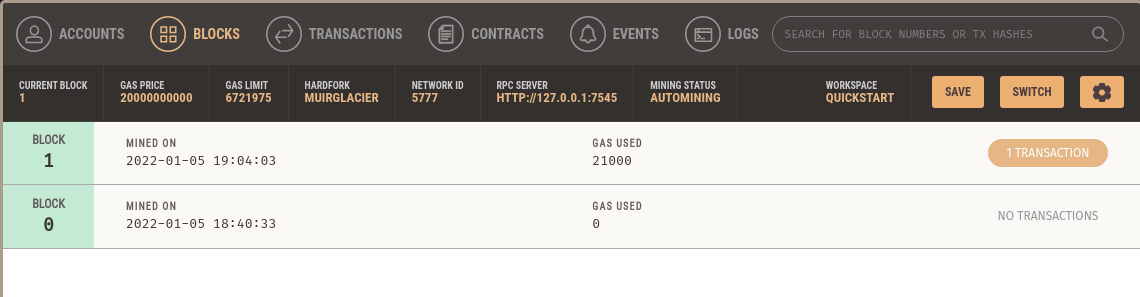
\includegraphics[width=0.8\textwidth]{ganache_block_mined.png}
    \caption{Example of Ganache blocks}
    \label{fig:1}
\end{figure}

\begin{figure}[H]
    \centering
    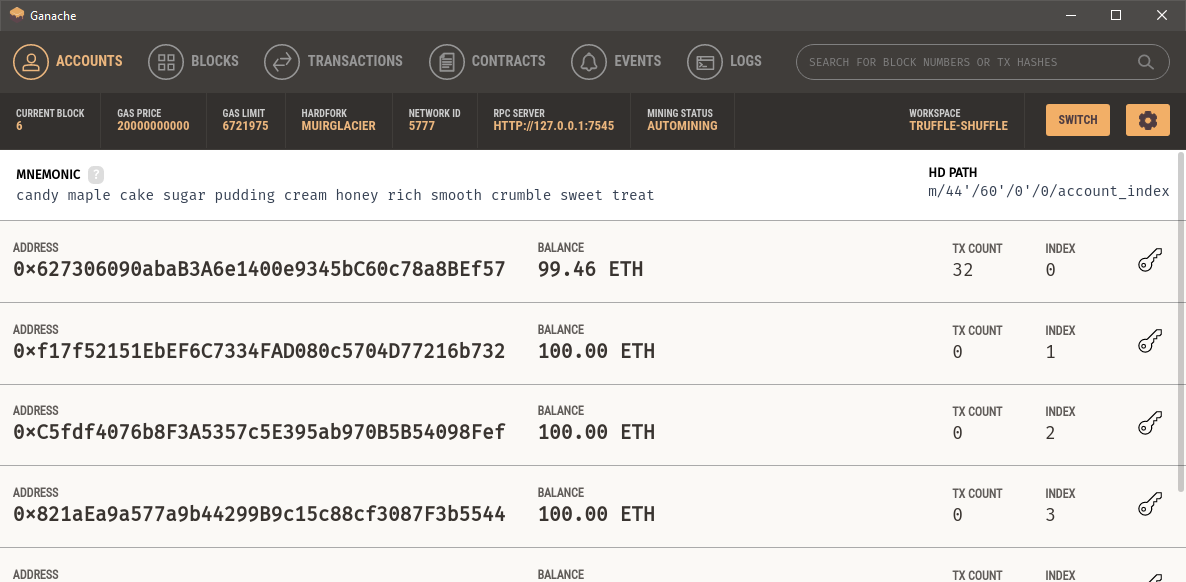
\includegraphics[width=0.8\textwidth]{ganache-window.png}
    \caption{Ganache - Truffle Suite}
    \label{fig:1}
\end{figure}
\section{Frequently Asked Questions}

\subsection{What is Ganache and how is it used in blockchain development?}

Ganache is a personal Ethereum blockchain used for testing and development. It allows developers to deploy, test, and debug smart contracts in a controlled environment without interacting with the main Ethereum network. Ganache provides a local blockchain with features such as:
\begin{itemize}
    \item Instant block mining, eliminating the need to wait for confirmations.
    \item Pre-funded accounts for easier testing.
    \item Detailed logging and debugging tools.
    \item Compatibility with Truffle Suite for streamlined smart contract deployment.
\end{itemize}

\subsection{What are the key differences between Ganache test network and the real Ethereum network structure?}

\begin{itemize}
    \item \textbf{Consensus Mechanism:} Ganache does not use Proof of Work (PoW) or Proof of Stake (PoS); blocks are mined instantly for testing purposes.
    \item \textbf{Gas Fees:} Transactions on Ganache do not require real gas fees, while on Ethereum, gas fees fluctuate based on network demand.
    \item \textbf{Block Time:} Ganache mines blocks immediately, whereas Ethereum has an average block time of 12–15 seconds (PoS).
    \item \textbf{Network Security:} Ganache operates locally and is not connected to public nodes, while Ethereum relies on a decentralized global network.
    \item \textbf{Persistence:} Data on Ganache resets when restarted unless explicitly saved, whereas Ethereum maintains a permanent ledger.
\end{itemize}

\subsection{How can you deploy a Solidity smart contract to a Ganache network using Truffle?}

To deploy a Solidity smart contract on Ganache using Truffle, follow these steps:

\begin{enumerate}
    \item \textbf{Install Truffle and Ganache:} 
    \begin{verbatim}
    npm install -g truffle
    \end{verbatim}
    \item \textbf{Initialize a Truffle project:} 
    \begin{verbatim}
    truffle init
    \end{verbatim}
    \item \textbf{Compile the smart contract:} Place the Solidity contract in the \texttt{contracts/} folder and run:
    \begin{verbatim}
    truffle compile
    \end{verbatim}
    \item \textbf{Configure the Truffle migration script:} Add a deployment script in the \texttt{migrations/} directory.
    \item \textbf{Start Ganache:} Run Ganache locally.
    \item \textbf{Deploy the contract:} Run the migration command:
    \begin{verbatim}
    truffle migrate --network development
    \end{verbatim}
    \item \textbf{Verify deployment:} Use Truffle console to interact with the deployed contract:
    \begin{verbatim}
    truffle console
    \end{verbatim}
\end{enumerate}

\subsection{What steps do you take to interact with a deployed smart contract on the Ganache network using Web3.js?}

To interact with a deployed smart contract using Web3.js, follow these steps:

\begin{enumerate}
    \item \textbf{Install Web3.js:} 
    \begin{verbatim}
    npm install web3
    \end{verbatim}
    \item \textbf{Connect to Ganache:} 
    \begin{verbatim}
    const Web3 = require('web3');
    const web3 = new Web3('http://127.0.0.1:7545'); // Default Ganache RPC URL
    \end{verbatim}
    \item \textbf{Load the smart contract ABI and address:} 
    \begin{verbatim}
    const contractABI = [ /* ABI JSON */ ];
    const contractAddress = '0xYourContractAddress';
    const contract = new web3.eth.Contract(contractABI, contractAddress);
    \end{verbatim}
    \item \textbf{Read contract data:} 
    \begin{verbatim}
    contract.methods.getValue().call().then(console.log);
    \end{verbatim}
    \item \textbf{Send a transaction:} 
    \begin{verbatim}
    contract.methods.setValue(42).send({ from: '0xYourAccountAddress' });
    \end{verbatim}
    \item \textbf{Listen for events:} 
    \begin{verbatim}
    contract.events.ValueChanged({}, (error, event) => {
        console.log(event);
    });
    \end{verbatim}
\end{enumerate}



\section{Conclusion}

In conclusion, Ganache serves as an invaluable tool for blockchain developers by providing a personal Ethereum blockchain for testing and development purposes. It simplifies the process of deploying, testing, and debugging smart contracts without the need to interact with the main Ethereum network. By using Ganache in conjunction with tools like Truffle and Web3.js, developers can create robust and secure smart contracts, ensuring their functionality before deploying them to a live environment. This controlled and efficient development workflow ultimately contributes to the advancement and reliability of blockchain
\
% \begin{figure}[H]
%     \centering
%     \includegraphics[width=0.8\textwidth]{}
%     \caption{}
%     \label{fig:1}
% \end{figure}


\clearpage
\begin{thebibliography}{99}
\bibitem{ganache}
Ganache - Truffle Suite. (n.d.). Retrieved from \url{https://www.trufflesuite.com/ganache}

\bibitem{truffle}
Truffle Suite. (n.d.). Retrieved from \url{https://www.trufflesuite.com/}

Web3.js - Ethereum JavaScript API. (n.d.). Retrieved from \url{https://web3js.readthedocs.io/}

\bibitem{ethereum}
Ethereum. (n.d.). Retrieved from \url{https://ethereum.org/}

\bibitem{solidity}
Solidity Documentation. (n.d.). Retrieved from \url{https://docs.soliditylang.org/}
\bibitem{web3js}
\end{thebibliography}

\end{document}